% Chapter 3

\chapter{GNSS实时滤波精密轨道确定的研究与实现}

\section{引言}

不论是提供事后或是实时的导航卫星轨道的位置服务,目前主流的GNSS精密轨道处理的方式仍是基于事后批处理的解算模型,其算法模型和处理流程随着多年来研究已经逐步趋于完善。相对的,基于实时观测数据,采用实时滤波解算方式进行轨道确定的处理模式在近几年仍在不断的研究和探索中。在事后批处理过程中,由于包含了所有观测数据信息,因此可以对观测数据进行统一的预处理,同时在解算过程中进行反复迭代计算和整体质量控制,以达到最优的数据处理效果。而实时滤波处理流程中往往需要通过处理实时观测数据流,实时给出当前已有观测数据信息下的最优轨道位置信息。因此实时滤波精密轨道确定在不论是在观测数据的预处理、参数估计方法、质量控制方法以及整体算法流程都与事后解算模式大不相同。如果直接应用事后解算模式的经验与方法,将难以取得理想的解算效果。

本章从实时滤波精密轨道确定的算法流程出发,分别对处理过程中的关键环节:参数估计方法、实时质量控制方法和实时模糊度固定方法,进行了相应的推导和实现,并通过实验对比分析验证了算法的正确性和有效性。最后,本文在目前已有的数据处理软件平台上GREAT(GNSS+ Research,
Application and Teaching)的基础上,开发实现了具有GNSS实时滤波精密轨道确定的功能,并给出了该功能的整体结构组成及其算法处理流程。

\section{基于平方根信息滤波的参数估计原理}

在第二章的参数估计部分,我们介绍了常用的最小二乘算法和卡尔曼滤波估计算法。其中卡尔曼滤波估计算法更适合实时数据的处理,相对于最小二乘批处理需要存储所有的观测值信息,滤波估计算法无需存储历史时刻的观测数据信息,而是以待估参数的协方差矩阵信息进行存储。同时滤波算法在处理具有先验运动模型的最优估计问题也更为直观。但由于计算机中计算过程截断误差的存在,导致存在滤波因数值误差而发散的情况存在,因此引入了平方根滤波相关的算法(Dyer,1969),其核心原理通过采用原有滤波算法一半字节长度进行相关数据信息的存储,大大减少了数值计算误差,从而抑制了滤波发散的情况,具有更高的数值稳定性。这里,我们选用了实时滤波轨道处理中常用的平方根信息滤波(Square Root Information Filter,SRIF)作为参数估计的方法。由于广义最小二乘算法在测绘领域更为常用,因此本文从广义最小二乘算法角度出发,推导和梳理了SRIF算法过程。

\subsection{量测更新算法}

对于已经构建好线性化后的观测函数模型以及确定了待估参数的问题中,最小二乘算法所求解的核心问题为:在包含有多余观测量的情况下,求解出一组最优的待估参数,使得所有观测方程的残差平方和最小,即满足式\eqref{eq:define_LSQ}。
    \begin{equation}
        \begin{aligned}
		& \nu = A_{m\times{n}}x_{n\times{1}}-b_{m\times{1}},P \\
		& \nu^{T}P\nu=min
        \end{aligned}
        \label{eq:define_LSQ}
    \end{equation}
式中,\(x\)为待估计的参数向量,\(A\)为观测函数模型化对在参数初始值上的线性化后的系数矩阵,\(b\)为观测值与使用参数初值计算的观测函数初值之差得到的先验残差向量。\(m,n\)分别为观测方程的数量与待估参数的维度。\(P\)为观测方程的权矩阵,这里假定其为正定对称阵。在此基础上,除考虑观测信息外,还需要考虑到待估计参数具有先验信息\(W\)。这里广义最小二乘算法的常见做法是构建基于先验的虚拟观测方程,和其他观测方程一同求解,即式\eqref{eq:define_LSQ}可以被扩展成式\eqref{eq:LSQ_more}。
    \begin{equation}
        \begin{aligned}
		& \nu =A_{new}x-b_{new},P_{new} \\ 
		& A_{new} = 
		\begin{bmatrix}
			E \\
			A 
		\end{bmatrix},
		b_{new} = 
		\begin{bmatrix}
			\bar{x}\\
			b
		\end{bmatrix},
		P_{new}=
		\begin{bmatrix}
			W & 0 \\
			0 & P
		\end{bmatrix}\\
        \end{aligned}
        \label{eq:LSQ_more}
    \end{equation}
式中,\(E\)为单位阵,\(\bar{x}\)为待估参数的先验值。

这里为了求解式\eqref{eq:LSQ_more},可以等价求解其对应的正规方程(normal equations),即\(A^{T}PAx=A^{T}Pb\)。当观测系统存在病态观测的时候,也就是系数矩阵\(A\)的条件数较大的时候,容易导致所求解的参数数值误差较大。为了避免这种情况,可以使用QR分解的方式进行求解。在使用QR分解算法之前,需要对上述广义最小二乘问题进行单位权规整化。对于前述的观测方程权矩阵和先验信息的权矩阵作三角化分解有,\(P=\varepsilon_{k}^{T}\varepsilon_{k},W=R_{k}^TR_{k}\),这里我们用下标\(k\)表明权矩阵所在时刻,因此,上述最小二乘问题可被等价转换为下面的表达:
\begin{equation}
	\begin{aligned}
	& min(\nu^{T}P\nu) =min \Vert Hx-l \Vert_{2} \\
	& H = 
	\begin{bmatrix}
		\varepsilon_{k}\\
		R_{k}A 
	\end{bmatrix}x ,
	l = 
	\begin{bmatrix}
		\varepsilon_{k}\bar{x} \\
		R_{k}b 
	\end{bmatrix}
	\end{aligned}
	\label{eq:LSQ_single}	
\end{equation}
式中,\(H,l\)分别表示规整化后的系数矩阵与先验残差向量。对系数矩阵进行QR分解有:
\begin{equation}
	\begin{aligned}
		& H_{m \times n}=
		\begin{bmatrix}
		\varepsilon_{k,m \times n}\\
		R_{k}A_{(m-n) \times n }
		\end{bmatrix} = 
		Q_{m \times m}
		\begin{bmatrix}
		\varepsilon_{k+1/k,m \times n}\\
		0_{(m-n) \times n}
		\end{bmatrix} \\ 
		& QQ^{T}=E
	\end{aligned}
	\label{eq:QR_factor}
\end{equation}
式中,\(Q\)为分解得到的正交矩阵。对式\eqref{eq:LSQ_single} 左右两边同乘以\(Q^{T}\),则可以得到相应的等价表达:
\begin{equation}
	\begin{aligned}
		min \Vert Hx-l \Vert_{2} & = min(\Vert
		\begin{bmatrix}
			\varepsilon_{k+1/k} \\
			0
		\end{bmatrix} x-Q^{T}
		\begin{bmatrix}
			\varepsilon_{k}\bar{x} \\
			R_{k}b 
		\end{bmatrix}
		 \Vert _{2})\\
		& = min(\Vert \varepsilon_{k+1/k}x - z \Vert_{2} +
			\Vert e \Vert_{2}
		)\\		
		& = min(\Vert \varepsilon_{k+1/k}x - z \Vert_{2}) \\
		z = Q^{T}\varepsilon_{k}\bar{x},
		e= Q^{T}R_{k}b
	\end{aligned} 
	\label{eq:SRIF_meqsuare_update}
\end{equation}
式中,\(e\)为正规化后的验后观测残差向量。此时待估参数可以直接用由\(\varepsilon_{k+1/k}^{-1}x=z\)直接求解得到,该方程在SRIF中也也被称为信息方程。到可以发现此表达式与k时刻的规整化的先验信息虚拟观测方程类似,此时\(\varepsilon_{k+1/k}^{T}\varepsilon_{k+1/k}\)即为求解后参数\(x\)的信息权矩阵,这里我们已经完成了SIRF量测更新的推导。在SRIF中,\(\varepsilon\)为待估参数的信息矩阵,因为其为原有的先验信息权矩阵三角化后的结果,在数值计算上具有更好的稳定性,其量测更新的核心原理即为式\eqref{eq:QR_factor},其中分解得到\(\varepsilon_{k+1/k}\)即可直接作为量测更新后参数的信息矩阵。

\subsection{时间更新算法}

导航卫星精密轨道确定问题中包含着大量的随时间变化的动态参数,如轨道参数、钟差参数、对流层参数和模糊度参数等。
如何在SRIF算法中随时间动态更新调整这些参数,也是实时滤波轨道处理中的一个关键步骤。
尽管这些动态参数各自具有不同的特性,但考虑它们一般化的时间更新过程,都包含了参数增加、参数状态更新、参数消除这三个部分。
接下来依次对这三个部分的具体算法流程进行相应的介绍

考虑j时刻的信息方程为\(\varepsilon_{j}x=z_{j}\)。其中,我们将参数\(x\)中分为两个类别\(x^{T}=[x_{r,j},x_{c}]\),其中\(x_{r,j}\)表示过了j时刻后需要消除的参数,\(x_{c}\)表示过了j时刻还需要保留的参数。假定\(\varepsilon_{j}\)的信息矩阵为上三角阵(若不为上三角阵,可做一次QR分解后得到),此时信息方程可表示为如下形式:
\begin{equation}
	\begin{aligned}
		\begin{bmatrix}
			\varepsilon_{r,j} & \varepsilon_{rc,j} \\
			0 & \varepsilon_{c,j} \\
		\end{bmatrix}
		\begin{bmatrix}
			x_{r,j} \\
			x_{c,j}
		\end{bmatrix}
		 =
		\begin{bmatrix}
			z_{r,j} \\
			z_{c,j} \\	
		\end{bmatrix}
	\end{aligned}
\end{equation}
对于下个历元新增加的参数这里我们使用\(x_{n,j+1}\)进行表示。对于新增参数,考虑其具有的先验信息方程为\(\zeta_{j+1}x_{n,j+1}=z_{n,j+1}\)。因此根据类似式\eqref{eq:LSQ_more}的广义最小二乘原理,此时参数增加后的信息方程可以直接表示为如下形式:
\begin{equation}
	\begin{aligned}
		\begin{bmatrix}
		\varepsilon_{r,j} & \varepsilon_{rc,j} & 0 \\
		0 & \varepsilon_{c,j} & 0 \\
		0 & 0 & \zeta_{j+1} 
		\end{bmatrix}				
		\begin{bmatrix}
			x_{r,j}\\
			x_{c,j}\\
			x_{n,j+1}
		\end{bmatrix}	
		=
		\begin{bmatrix}
			z_{r,j}\\
			z_{c,j}\\
			z_{n,j+1}
		\end{bmatrix}
	\end{aligned}
	\label{eq:init_eq}
\end{equation}

考虑到\(x_{r,j}\)和\(x_{n,j+1}\)可以构建如下的状态变化方程:
\begin{equation}
	\begin{aligned}
	& x_{n,j+1} = \phi_{j+1/j}x_{r,j}+ \beta_{j+1/j},W_{\omega}   \\ 
	& W_{\omega}=R_{\omega}^{T}R_{\omega}
	\end{aligned}
	\label{eq:trans_eq}
\end{equation}
式中,\(\phi_{j+1/j}\)为线性化后的状态转移矩阵,\(W_{\omega}\)为状态转移方程的信息权矩阵,其三角化分解后的结果为\(R_{\omega}\),\(\beta_{j+1}\)为状态转移方程中的过程噪声,其大小一般与状态转移的时间间隔相关。
到这里可以发现,本质上完成参数的状态更新过程,即等价于将式\eqref{eq:trans_eq}当作观测方程,对式\eqref{eq:init_eq}的信息方程完成一次量测更新。因此对参数进行状态更新依然可以基于QR分解完成。这里我们仿照式\eqref{eq:LSQ_single}构造如下的最小二乘模型,并对系数矩阵进行QR分解,可以得到如式\eqref{eq:SRIF_timeupdate}的形式:
\begin{equation}
  \begin{aligned}
	 min(\Vert Hx-l \Vert_{2}) & = min(\Vert
	 \begin{bmatrix}
		\varepsilon_{r,j} & \varepsilon_{rc,j} & 0 \\
		0 & \varepsilon_{c,j} & 0 \\
		0 & 0 & \zeta_{j+1} \\
		-R_{\omega}\phi & 0 & R_{\omega}\\
	\end{bmatrix}
	\begin{bmatrix}
		x_{r,j}\\
		x_{c,j}\\
		x_{n,j+1}
	\end{bmatrix}
	-
	\begin{bmatrix}
		z_{r,j}\\
		z_{c,j}\\
		z_{n,j+1} \\
		R_{\omega}\beta_{j+1/j}
	\end{bmatrix}
	\Vert_{2} )\\
	& \Downarrow H = QR \\
	& = min(\Vert 
	\begin{bmatrix}
	\varepsilon_{r,j+1} & \varepsilon_{rc,j+1} & \varepsilon_{rn,j+1} \\
	0 & \varepsilon_{c,j+1} & \varepsilon_{cn,j+1} \\
	0 & 0 & \varepsilon_{n,j+1}\\
	0 & 0 & 0
	\end{bmatrix}
	\begin{bmatrix}
		x_{r,j}\\
		x_{c,j}\\
		x_{n,j+1}
	\end{bmatrix}
	-
	Q^{T}
	\begin{bmatrix}
		z_{r,j}\\
		z_{c,j}\\
		z_{n,j+1} \\
		R_{\omega}\beta_{j+1/j}
	\end{bmatrix}
	\Vert_{2})
  \end{aligned}	
  \label{eq:SRIF_timeupdate}
\end{equation}
式中,\(\varepsilon_{j+1}\)表示了j+1时刻下的信息方程的信息矩阵,\(Q\)为对系数矩阵进行QR分解得到的正交矩阵。这样便推导得到了参数状态过更新后的信息方程。
最后,可以发现由于信息矩阵为上三角矩阵,对于后续不再需要的\(x_{r,j}\)参数,可以很自然地将其对应的信息方程中的所在行删除,方程剩余的部分依然满足信息方程的结构。
同时,由于SRIF算法中的时间更新和量测更新是随时间不断地迭代进行,因此删除过时参数可以大大避免因为这些参数导致的无意义的计算资源的消耗。

至此,已经推导得到了基于QR分解实现时间更新基本原理。对于参数增加和消除,由于信息方程的上三角化的特殊结构,可以通过简单的矩阵变换得到。
对于参数状态更新的部分,其核心关键就在于构建式\eqref{eq:trans_eq}的状态转移方程以及式\eqref{eq:SRIF_timeupdate}的信息方程的时间更新。

\subsection{基于SRIF的实时滤波轨道处理流程}
\begin{figure}
  \centering
  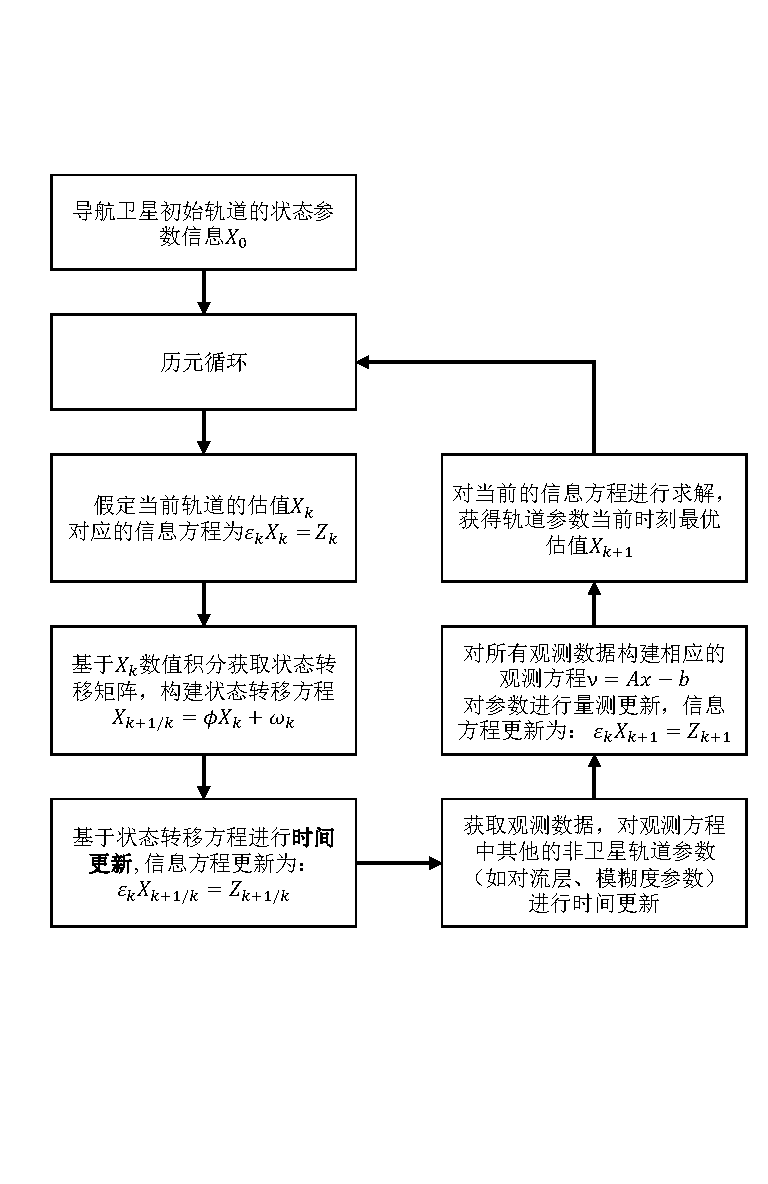
\includegraphics{SRIF_flowchart.pdf}
  \caption{基于SRIF的实时滤波轨道处理流程图}
  \label{fig:SRIF_flowchart}
\end{figure}
前面推导了平方根信息滤波的量测更新和时间更新的基本原理,图~\ref{fig:SRIF_flowchart}给出了出基于平方根信息滤波的实时滤波轨道的基本处理流程。
首先,这里将实时滤波轨道中的时间更新分成了轨道参数与其他参数两个部分。
其中,对于轨道参数的更新,我们通常需要通过数值积分获取前后历元的状态转移矩阵,从而构建相应的状态转移方程。但考虑到数值积分过程较为耗时,这里通常不需要在每个历元进行积分计算,而是使用之前数值积分的计算结果作一个近似处理。
对于状态转移方程的构建,本文采用随机游走的函数模型(Random Walk,RW)来进行描述。假定导航卫星的速度参数和动力学模型参数的误差为零均值白噪声(White Noise,WN)模型(这里我们忽略了动力学模型参数误差对速度误差造成的影响),因此对于前后时间间隔为\(\Delta t\)的轨道参数状态转移方程,其协方差矩阵(其值和信息权矩阵为互逆关系)为下式\eqref{eq:trans_eq_W}所示。
\begin{equation}
	\begin{aligned}
		W(orb)^{-1}=
		\begin{bmatrix}
			\frac{\Delta t^{3}}{3}\sigma^{2}E_{3\times3} & 
			\frac{\Delta t^{2}}{2}\sigma^{2}E_{3\times3} &
			0_{3\times n_{q}} \\
			\frac{\Delta t^{2}}{2}\sigma^{2}E_{3\times3} & 
			\Delta t\sigma^{2}E_{3\times3} &
			0_{3\times n_{q}} \\
			0_{3\times n_{q}} &
			0_{3\times n_{q}} &
			\sigma_{q}^{2}E_{n_{q}\times n_{q}} \\
		\end{bmatrix}
	\end{aligned}	
	\label{eq:trans_eq_W}
\end{equation}
式中,\(\sigma^{2}\)和\(\sigma_{q}^{2}\)分别表示了表示导航卫星速度误差和导航卫星动力学模型噪声的白噪声方差,具体实现则采用了经验值
\(10^{-12}\)和\(10^{-14}\)(参考文献xxxx)。
由于在平方根滤波中,需要对方程进行单位权标准化,因此我们通常使用其三角化后的结果,即如下式\eqref{eq:trans_eq_RW}所示:
\begin{equation}
	\begin{aligned}
		&R(orb)^{T}R(orb)=W(orb) \\
		& R(orb) =
		\begin{bmatrix}
			\frac{2\sqrt{3}}{\Delta t^{\frac{3}{2}}\sigma^{2}}E_{3\times3} & 
			\frac{-\sqrt{3}}{\Delta t^{\frac{1}{2}}\sigma^{2}}E_{3\times3} &
			0_{3\times n_{q}} \\
			0_{3\times 3} &
			\frac{1}{\Delta t^{\frac{1}{2}}}E_{3\times3} &
			0_{3\times n_{q}} \\
			0_{3\times n_{q}} &
			0_{3\times n_{q}} &
			\frac{1}{\sigma_{q}^{2}}E_{n_{q}\times n_{q}} \\
		\end{bmatrix}
	\end{aligned}	
	\label{eq:trans_eq_RW}
\end{equation}

而对于非轨道参数的更新,在无电离层模型中,主要需要考虑钟差参数、对流层参数、系统间偏差参数和模糊度参数的状态更新。对于钟差参数和模糊度参数,通常直接采用WN模型进行估计,因此在时间更新过程中只需要考虑参数增加和参数消除的步骤;
而对于系统间偏差参数和对流层参数则采用分段常数的模型进行估计。其中系统间偏差考虑其随时间变换较为稳定,可以按每天分段,而对流层参数则相对更新更为频繁,可以按每两个小时进行分段。

完成所有参数的时间更新后,根据当前历元的观测数据构建相应的观测方程,即可进行SRIF的量测更新。通常,我们不直接估计待估参数的绝对量,而是估计相对于初值的改正量。尽管量测更新后已经可以得到待估参数的最优估计值,但并不能直接将其更新为新的初值进行滤波后续的更新,因为更新前后待估参数的所估计的改正量相对的初值已经不一致了,其参数含义已经发生了改变。对于所选取初值较为准确或者线性化误差影响小的参数(如钟差、模糊度参数),可以选择继续沿用之前的初值进行滤波的后续处理。而对于线性化误差影响较大的参数(如轨道参数),则应当对这些参数做一次时间更新,其中,状态方程为如下式\eqref{eq:SRIF_zero_noise}所示:
\begin{equation}
	\begin{aligned}
		x_{t} - x_{t+1} = \overline{x_{t}}_{0} - \overline{x_{t+1}}_{0},P_{t+1/t}=\infty
	\end{aligned}
	\label{eq:SRIF_zero_noise}	
\end{equation}
式中,\(x_{t}\)表示t时刻的待估参数,\(x_{t+1}\)表示初值更新后t+1时刻的待估参数\(P_{t+1/t}\)表示这个状态方程的信息权。由于本质上两个参数仅仅是初值不一致,其状态方程的噪声应为0,即信息权为\(\infty\),因此无法按一般方法直接进行时间更新。这里可以通过对原有参数做一次线性变换以此等价实现信息权为\(\infty\)的时间更新。这里考虑具有如下一般形式的状态方程:
\begin{equation}
	\begin{aligned}
		Ax_{t} - Bx_{t+1} = l_{t+1/t}
	\end{aligned}
	\label{eq:SRIF_zero_trans_eq}	
\end{equation}
考虑对于\(x_{t}\)参数具有如下的信息方程:
\begin{equation}
	\varepsilon_{t}x_{t}=z_{t}
	\label{eq:SRIF_zero_trans_eq2}
\end{equation}
将式\eqref{eq:SRIF_zero_trans_eq}带入式\eqref{eq:SRIF_zero_trans_eq2}即可以对信息方程完成如下的更新:
\begin{equation}
	\begin{aligned}
	& x_{t} = A^{-1}BX_{t+1}+A^{-1}l_{t+1/t}\\
	& \varepsilon_{t+1}x_{t+1}=z_{t+1}\\
	& \varepsilon_{t+1}=\varepsilon_{t}A^{-1}B\\
	& z_{t+1}=z_{t}-\varepsilon{t}A^{-1}l_{t+1/t}
	\end{aligned}
\end{equation}
式中也是给出对于间更新过程中的状态方程设定极小噪声的方法。由于计算机数值误差的原因,设置过大的信息权阵依然会引起SRIF滤波器的发散现象,采用上述的转换,可以实现接近的更新。

\section{GNSS实时数据精化}
上一节中我们阐述了SRIF滤波器在精密轨道确定中的使用方法,其中SRIF量测更新过程成立的前提是假定了参与更新的观测方程的观测噪声满足高斯正态分布的随机模型。因此若要确保SRIF滤波器能够得到正确的估计结果,需要尽可能的保证输入的是“干净”的观测值,否则其中的“异常值”将会导致滤波器收敛速度减缓甚至发散。
由于GNSS信号传播过程会受到外界环境因素(如多路径效应、大气环境不稳定、接发硬件因素)等影响,导致大量GNSS观测数据中包含异常观测值的概率并不低。特别地,对于GNSS观测值中的相位观测值,由于本身的特性,还存在着整周跳变(周跳)的问题,这严重影响着观测值得精度水平。因而需要对GNSS异常值进行有效地探测和剔除。
在精密轨道确定事后批处理的模式中,其对GNSS异常值的处理,通常会在参数估计前对观测数据进行整体预处理,以及在参数估计后利用观测方程的验后残差进行相应的探测。
类似地,实时滤波轨道中同样可以在SRIF量测更新前后,分别对GNSS数据质量进行相应的检测。接下来依次对这两部分所采用的算法模型和处理策略进行介绍。

\subsection{实时数据质量检测算法}
考虑到GNSS载波相位观测值具有较高地量测精度,其很大程度决定着数据处理的最终精度,因此有效地探测其本身的粗差和周跳对GNSS数据处理至关重要。
Turboedit方法(Blewit,1990)是目前被广泛应用的载波相位观测值质量检测算法,实时滤波轨道处理中同样使用了该方法对载波相位观测值进行检测。其基本思想是通过构造Melbourne-Wubbena(MW)双频组合观测值和无几何距离(Geometry-Free,GF)组合观测值,设定相应的阈值,对连续时间内的组合观测值序列进行分析,从而筛选出包含周跳或粗差的观测值。同时对于GNSS实时数据,由于其处理具有不可逆性,因此不能直接对整个弧段内的观测值序列直接进行分析,需要在原有基础上进行改进,以适应实时处理过程(张小红等,2010)。具体的算法流程如下,这里我们使用\(f_{1},f_{2}\)表示观测值所采用的频率,\(L,P\)分别表示相位和伪距观测值。
因此GF组合观测值可以被表达为如下形式:
\begin{equation}
	\begin{aligned}
		L_{GF}=L_{1}-L_{2}=I_{12}+\lambda_{1}N_{1}-\lambda_{2}N_{2}	
	\end{aligned}
	\label{eq:GF_eq}
\end{equation}
式中,\(I_{12}\)表示电离层延迟在两个频率观测上的差值,\(N\)表示模糊度,\(\lambda_{1},\lambda_{2}\)分别表示对应频率的波长。可以看到\(L_{GF}\)不随几何距离发生改变,且在模糊度未发生周跳的情况下,其仅随电离层延迟之差的变化而改变。则GF观测值的前后历元差值可以表达为:
\begin{equation}
	\begin{aligned}
	\Delta L_{GF}(t,t+1) = \Delta I_{12}(t,t+1) + \lambda_{1}\Delta N_{1}(t,t+1) - \lambda_{2}\Delta N_{2}(t,t+1)
	\end{aligned}
	\label{eq:GF_delta}
\end{equation}
其中电离层延迟随时间变化缓慢,\(\Delta I_{12}(t,t+1)\)接近于0,因此\(\Delta L_{GF}\)可以作为判断模糊度周跳判断的依据。在模糊度没有发生周跳的情况下,\(\Delta L_{GF}\)通常在厘米级别波动。
考虑到精密轨道确定中的时间采样间隔一般相对较长(300s为例),可以选取经验阈值为15cm。在实际处理中,低高度角的观测数据由于多路径效应等原因其观测噪声相对更大,应适当放松判断阈值。本文中所采用的阈值模型具体如下所示:
\begin{equation}
	\begin{aligned}
		& \Delta L_{GF}(t,t+1) < l * Limit_{GF},Lmit_{GF}=0.15m\\
		& l=
		\begin{cases}
			  2- \frac{\theta}{15.0} & \theta < 15.0 \\
			  1 & \theta >=15.0 \\
		\end{cases}
	\end{aligned}
\end{equation}
式中,\(\theta\)表示观测数据的卫星高度角。GF组合观测值判断周跳成功的前提是在电离层活动平静,延迟变化缓慢,同时对于特殊的双频周跳组合也存在探测盲区。因此还需要借助MW组合观测值进行进一步的判断。MW组合观测值可以表达为如下形式:
\begin{equation}
	\begin{aligned}
		 N_{WL} & =\frac{L_{1}}{f_{1}}-\frac{L_{2}}{f_{2}}-\frac{f_{1}P_{1}+f_{2}P_{2}}{\lambda_{WL}(f_{1}+f_{2})} \\
		& = N_{1}-N_{2}\\
	\end{aligned}	
\end{equation}
式中,\(N_{WL}\)为MW组合观测值,也称为宽巷模糊度。可以看到其值为两个频率上的模糊度的直接差值,在模糊度没有发生跳变的情况下,其前后历元MW组合观测值的差值\(\Delta N_{WL}\)应表现出零均值白噪声的特性。考虑到MW组合观测值的计算包含了伪距观测值,因此其中还包含了较大的伪距观测噪声,直接使用前后历元的比较结果受噪声影响较大,容易造成周跳的误判,因此常用一段时间的观测值对其进行相应的平滑。考虑到实时数据无法像事后处理存储所有的观测数据,这里需要采用滑动窗口的方式进行相应的计算,具体如下所示:
\begin{equation}
	\begin{aligned}
		& \overline{N_{WL}}=\frac{1}{win}\sum_{i=t-win}^{t}N_{WL}(i) \\ 
		& \sigma_{WL}=\sqrt{\frac{\sum_{i=t-win}^{t}(N_{WL}(i)-\overline{N_{WL}})^{2}}{win}} \\
	\end{aligned}
\end{equation}
式中,\(win\)表示了滑动窗口的大小,\(\overline{N_{WL}},\sigma_{WL}\)分别表示了MW组合观测值序列在滑动窗口内的均值和标准差。接着,可以构造如下的检验量:
\begin{equation}
	\begin{aligned}
		& \frac{N_{WL}-\overline{N_{WL}}}{\sigma_{WL}} < k\bullet Limit_{WL},Limit_{WL}=4 \\ 
		& k=\begin{cases}
			3-0.1\theta & \theta < 20.0 \\ 
			1 &  \theta >=20.0
		\end{cases}	
	\end{aligned}
\end{equation}
式中,\(Limit_{WL}\)为MW组合周跳判断的阈值,这里选用的为经验值,类似GF组合,同样采用了高度角阈值模型。尽管MW组合观测值同样存在的一定的探测盲区,但其与GF组合观测值结合可以互相消除各自的探测盲区,因此上述两种方法的同时使用基本可以探测出所有周跳情况。

对于GNSS伪距观测值,尽管精度相较相位观测值更低,但可以为GNSS方程提供钟差基准,同时对滤波器的收敛起主要作用。另外考虑到MW组合观测值中包含了伪距观测值,因此包含粗差的伪距观测值也会导致组合量阈值超限,进而造成一些相位观测值数据的浪费。
因此这里对伪距观测量进行一个粗略的质量检测,若探测为粗差则相应地放大MW组合观测值的判断阈值。具体的算法原理如下式\eqref{eq:preprocess_code}所示:1
\begin{equation}
	\begin{aligned}
		& \begin{aligned}
			 \Delta P(i,j)&=P_{i}-P_{j} \\
		& = d^{s}+d_{r}+d_{iono(i\not=j)}+\varsigma \\
		\end{aligned} \\
		& \Delta P(i,j) <Limit_{P}\\
		& Limit_{P} = \begin{cases}
			10 & i=j \\ 
			30 & i\not=j \\
		\end{cases}
	\end{aligned}
	\label{eq:preprocess_code}
\end{equation}
式中,\(i,j\)分别表示伪距观测值中所采用的频率,\(d^{s},d_{r}\)分别表示卫星端和接收机端的硬件延迟在不同频率或信号通道上的差值。\(d_{iono}\)表示不同频率的电离层延迟之差,\(\varsigma\)表示观测噪声之差。\(Limit_{P}\)为相应的判断阈值。考虑对同个频率不同信号通道上的观测值,其电离层延迟可以被消除,因此相对的其判断阈值小于不同频率的判断阈值。

综上所述,实时滤波轨道处理中实时数据处理检测的算法主要包括了伪距粗差探测和载波相位周跳探测,其中周跳探测部分则主要采用了结合GF组合观测值和MW组合观测进行联合判断的方式。整体的算法流程如下图~\ref{fig:tb_flowchart}所示:
\begin{figure}
  \centering
  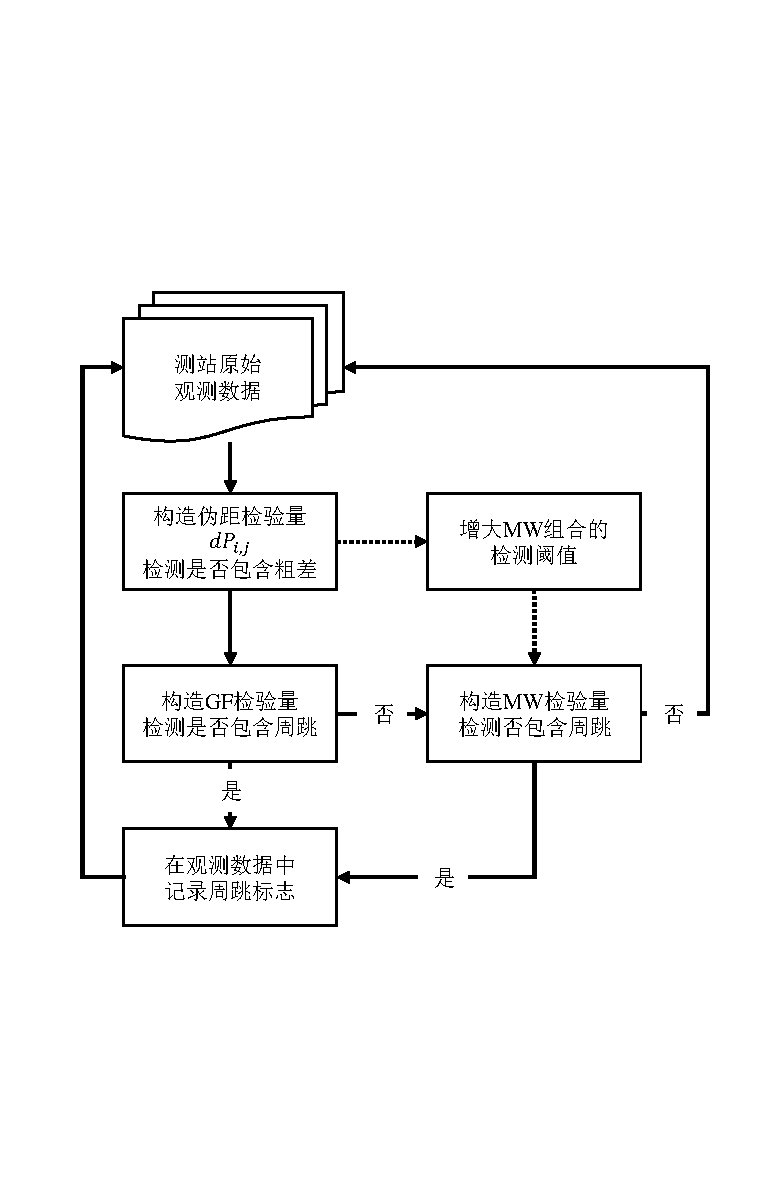
\includegraphics{preprocess.pdf}
  \caption{GNSS实时数据预处理算法流程图}
  \label{fig:tb_flowchart}
\end{figure}

\subsection{实时质量控制算法}
前一节当中所述的实时数据质量检测算法适用于参数估计前的一个初步质量控制,通常所设定的判断阈值相对较大,只能用于探测一些“大粗差”,而想要进行更为细致的质量控制,需要采用基于假设检验的数据质量探测方法,其中DIA质量控制方法是目前最为常用的方法。
其基本思想是针对参数估计后的观测方程延后残差构造检验量(通常为单位权中误差),通过卡方假设检验判断是否存在粗差。如果存在,则需要定位观测值中的粗差并剔除,并重新进行参数估计和假设检验,直至没有粗差为止。
基于平方根信息滤波的DIA质量控制方法与常见的最小二乘和卡尔曼滤波等最优估计方法具有一定的区别。相较于需要根据参数的估计值重新计算观测方程的验后残差,SRIF的量测更新后可以直接得到标准化的验后残差,同时在重新计算剔除粗差观测后的验后残差也更为简便。接下来将基于SRIF的质量控制算法分为探测粗差、确定粗差、剔除粗差三个部分,依次介绍。

首先是探测粗差。以式\eqref{eq:SRIF_meqsuare_update}中的SRIF量测更新方程为例,其等价表达如下:
\begin{equation}
	\begin{aligned}
		\begin{bmatrix}
			\varepsilon_{k+1/k} \\
			0
		\end{bmatrix} x&=Q^{T}
		\begin{bmatrix}
			\varepsilon_{k}\bar{x} \\
			R_{k}b 
		\end{bmatrix}\\
		& = \begin{bmatrix}
			Q_{par} &  Q_{obs}
		\end{bmatrix}	
		\begin{bmatrix}
			\overline{z}_{par} \\
			\overline{z}_{obs}
		\end{bmatrix}\\
		& =  \begin{bmatrix}
			z_{par} \\	
			e_{obs}
		\end{bmatrix}	
	\end{aligned}
\end{equation}
式中,\(\overline{z}_{par},\overline{z}_{obs}\)用于表示参数的先验信息,和观测方程标准化的先验残差。\(Q_{par},Q_{obs}\)分别表示对\(\overline{z}_{par},\overline{z}_{obs}\)的敏感矩阵,\(z_{par},e_{obs}\)分别表示量测更新后参数信息和标准化的验后残差。利用\(e_{obs}\)可以构造如下的检验量:
\begin{equation}
	\begin{aligned}
		& T= e_{obs}^{T}e_{obs} \sim \chi_{\alpha}^{2}(n_{obs},0) \\
		&max(e_{obs}) > Limit_{e},Limit_{e}=3.0
	\end{aligned}
\end{equation}
式中,\(\chi\)为卡方检验,\(\alpha\)为置信度,\(n_{obs}\)为观测方程数。除了通过检验量判断,还可以判断验后残差是否大于相应阈值。

接着是定位粗差。如果通过上面的步骤确认了观测值中存在相应的粗差。则可以对\(e_{obs}\)进行相应的排序,从大到小依次对各个观测值进行判断。假定当前观测值存在粗差\(\Delta z_{obs}\),一般而言可以通过舍弃观测值,或者新增该观测值的偏差参数来重新计算进行上个步骤的检验量。考虑到敏感矩阵\(Q_{obs}\)不随观测值发生改变,因此偏差参数可以直接表达为如下形式:
\begin{equation}
	\begin{aligned}
		 min & =||e_{obs}+Q_{obs}\Delta z_{obs}||^{2}\\
		& \Downarrow \\
		 \Delta z_{obs} & =(Q_{obs}^{T}Q_{obs})^{-1}Q_{obs}^{T}(-e_{obs})
	\end{aligned}	
	\label{eq:get_DeltaZ}
\end{equation}
得到偏差参数的估值后,即可以得到新的标准化验后残差。此时可以根据上一节中探测粗差的步骤重新进行判断,以此不断迭代探测出观测值中所有的异常值。

最后是剔除粗差。根据式\eqref{eq:get_DeltaZ}可以统一求出所有异常观测值的偏差参数,从而获得粗差剔除后的信息方程。同时在探测出的异常观测值中,对于伪距可以统计测站出现的频率,依次剔除部分数据观测较差的测站;对于相位观测值,一般将其认定发生了周跳,因此需要对相应的模糊度参数进行SRIF时间更新。

综上所述,基于平方根滤波算法的质量控制算法可以快速构造检验量并利用敏感矩阵对异常观测值的偏差量进行确定,其整体的算法流程如下图~\ref{fig:qc_flowchart}所示。

\begin{figure}
  \centering
  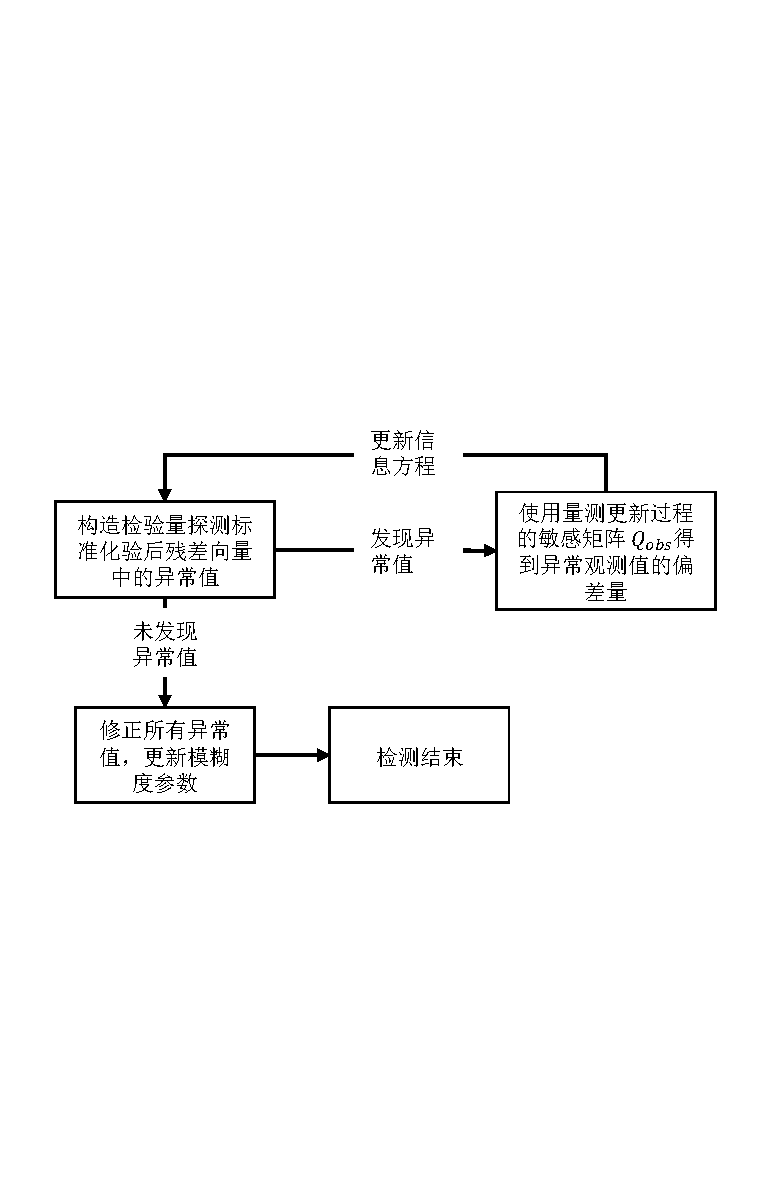
\includegraphics{qc_flowchart.pdf}
  \caption{GNSS实时数据预处理算法流程图}
  \label{fig:qc_flowchart}
\end{figure}

\subsection{实验结果和分析}
为了进一步验证上述实时数据质量检测算法的有效性,选用了事后数据进行了GPS系统这里选用经过精密定轨事后迭代出处理的数据质量控制文件作为参考,认为其中基本不存在粗差和周跳。

\begin{figure}
  \centering
  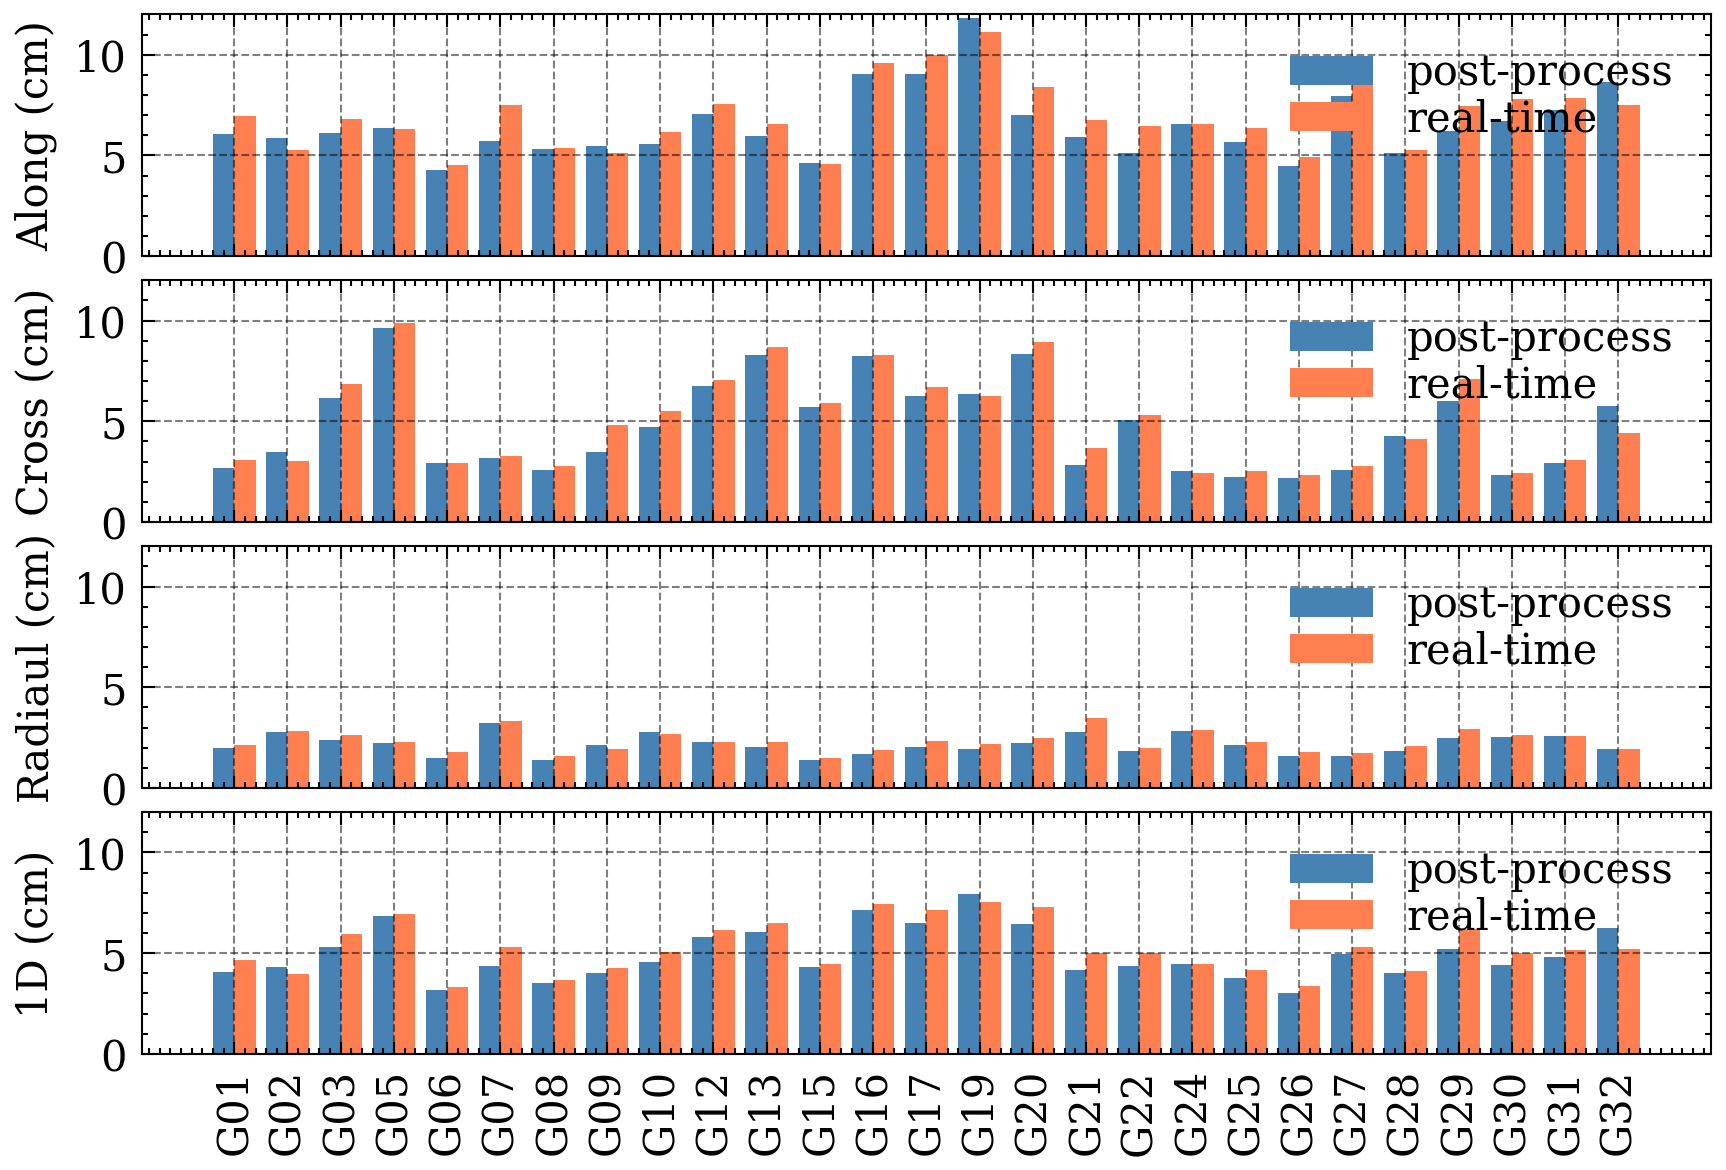
\includegraphics{srif_average_compare_logtb_litetbQC.png}
  \caption{GNSS实时数据预处理算法流程图}
  \label{fig:tbqc_compare}
\end{figure}

\begin{table}[ht]
  \centering
  \caption{GPS仿实时滤波浮点解与COD轨道产品比较平均RMS(cm)结果统计}
  \label{tab:tbqc_compare}
  \begin{tabular}{ccccc}
    \toprule
    Item & Along & Cross & Radiaul & 3D \\
    \midrule
	Post-Process QC & 6.4 & 4.7 & 2.1 & 8.6 \\
	Real-Time QC & 6.9 & 4.9 & 2.3 & 9.1 \\
	Dai-float & 6.1 & 4.7 & 3.0 & 8.3  \\
    \bottomrule
  \end{tabular}
\end{table}

\begin{figure}
  \centering
  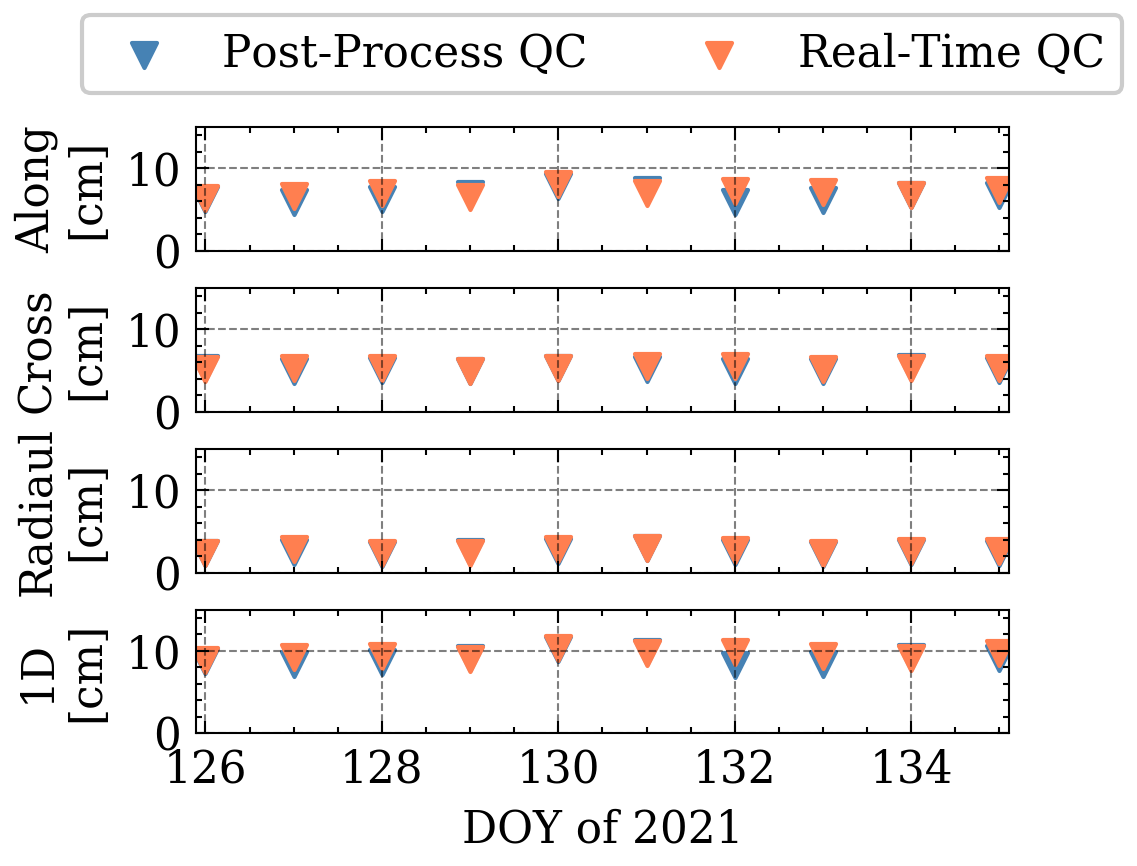
\includegraphics{srif_average_compare_logtb_litetbQC_series.png}
  \caption{GNSS实时数据预处理算法流程图}
  \label{fig:tbqc_compare_series}
\end{figure}


实验设计:

主要目的:选用经过多次迭代后的log\underline{\space}tb文件作为参考值,认为其中没有发生周跳。以此对比实时质量算法所起的作用。

分别使用该log\underline{\space}tb文件,以及实时周跳探测和质量控制的算法分别进行实时滤波轨道确定计算

实验方案: 110 个测站 10天的3d解(天数可以商榷) GPS单系统
方案1:使用log\underline{\space}tb进行计算(关掉了实时周跳探测以及实时质量控制,纯解算)

方案2:开启litetb(感觉需要使用300s的阈值,否则这样信息感觉比事后的tb解算多),其次是开启质量控制算法(即重置模糊度,这里需要测试不同max\_res\_norm阈值下的结果吗 这个感觉有点区别啊)

\section{实时双差模糊度固定方法}

\subsection{双差模糊度固定算法基本原理}

\subsection{实验结果和分析}

实验设计:

主要目的:
相较于浮点解,对比不同模糊度固定算法在实时轨道中所起的作用

实验方案:110个测站  10天的3d解,基于编辑残差后的log\_tb进行解算结果? GCE三系统的结果
同时对比不同的实验方案(紧约束的和松约束)

这里就直接说是基于残差log\_tb的结果算了,不过实际算的时候应该使用初始tb加上实时质量控制的算法

\section{实时滤波精密轨道处理软件结构}

画图画图再画图
